\chapter{指数・対数}\label{chapt_exp_log}
{\small 過去の受講生の言葉: 「最近ようやく定義を1つずつ確認する癖がつき, 理解しやすくなった。」}

%{\small 基礎がしっかりしていて, 子供のようなミスは決して犯さない。
%それが真剣さというものだ (イビチャ・オシム 元サッカー日本代表監督)。\\}

\section{指数関数}

$a$を正の定数とし, $a^x$という関数を考えよう。こういう関数を
\underline{指数関数}\index{しすうかんすう@指数関数}という。例えば$a=2$のときは, 
$2^x$であり, これは$x=0, 1, 2, 3, 4$のときは
それぞれ, 1, 2, 4, 8, 16, ...と, 急速に大きくなる。パソコンを使って
$y=2^x$をグラフに描くと, \fref{fig:y2powx}の実線のようになる。
\begin{figure}[h]
    \centering
    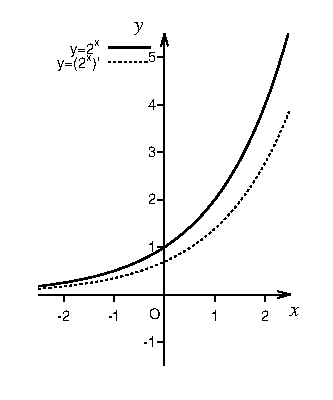
\includegraphics[width=6.0cm]{y2powx.eps}
    \caption{$y=2^x$と$y=(2^x)'$のグラフ}\label{fig:y2powx}
\end{figure}
ここで, $y=2^x$を数値微分した結果(つまり導関数)も点線で描いた。
これを見ると, $y=2^x$とその導関数はちょっと似ている。それは, 
$y=2^x$が急激な右肩上がりの曲線なので, 右に行くほど接線の
傾きも急速に大きくなる, 従って, 導関数(接線の傾きの値を
並べたもの)も右肩上がりになるのだ。

では, 同じようなことを$y=3^x$についてやってみたらどうだろう?
結果は, \fref{fig:y3powx}のようになる。
\begin{figure}[h]
    \centering
    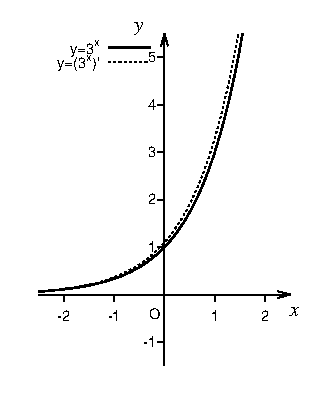
\includegraphics[width=6.0cm]{y3powx.eps}
    \caption{$y=3^x$と$y=(3^x)'$のグラフ}\label{fig:y3powx}
\end{figure}
やはり, $y=3^x$は急激に右肩上がりの曲線で, その導関数も似ている。
\fref{fig:y2powx}と\fref{fig:y3powx}を比べてみると, 
\fref{fig:y3powx}の方が, もとの関数と導関数はずっと近い。しかし, 
\fref{fig:y2powx}ではもとの関数よりも導関数の方が下にあったのが, 
\fref{fig:y3powx}ではやや上にある。ということは, $a$が3よりも若干
小さい数では, $y=a^x$とその導関数がぴったり一致するのではない
だろうか? 実はそうなのである。いろいろ試すと, $a$が$2.71828\cdots$
のときにそうなるのだ。これが, \pref{eq:NapierNum_value}
で出てきた\underline{ネイピア数}\index{ねいぴあすう@ネイピア数}$e$の正体である。すなわち, 
\begin{eqnarray}
(e^x)'=e^x\label{eq:exp_diff}
\end{eqnarray}
となるような数$e$をネイピア数と言うのだ。そして, $e^x$は, 
「微分しても変わらない指数関数」である。$e^x$のことを, \underline{エクスポーネンシャル} 
(exponential)\index{えくすぽーねんしゃる@エクスポーネンシャル} と呼ぶ。
なお, 第1章で述べたように, $e^x$を, $\exp x$\index{exp}と書くことも多い。
単なる書き方の約束だが, 意外に見落とす人がいるので, もういちど大きく書いておこう:

\begin{itembox}{約束}
\begin{eqnarray}\exp x :=e^x\end{eqnarray}
\end{itembox}

\begin{q}\label{q:exp_graph0} 表計算ソフトで, $y=2.718^x$のグラフと, 
$y=2.718^x$を数値微分したグラフを, 重ねて描いてプリントアウトせよ。$x$の
刻みは0.01くらいでよい。$x$の範囲は$-2$以上2以下としよう。\end{q}

実は, ネイピア数$e$は, 次式を満たす:
\footnote{$dx$を微小量とする。$e$が$(e^x)'=e^x$を満たすなら, 
微分の定義より, $e^{x+dx}=e^x+e^xdx$のはず。従って, 
$e^{x+dx}=e^x(1+dx)$。一方, 指数法則より, $e^{x+dx}=e^xe^{dx}$。
これらを比べて, $e^{dx}=1+dx$。両辺を$1/dx$乗して, $e=(1+dx)^{1/dx}$。
$dx$を$h$に置き換えたら\eref{eq:def_NapierNum0}になる。}
\begin{eqnarray}
e=\lim_{ h \to 0} ( 1 + h)^{1/h}\label{eq:def_NapierNum0}
\end{eqnarray}
あるいは, $1/h$を$n$と置き換えて, 
\begin{eqnarray}
e=\lim_{n \to \infty} \Bigl( 1 + \frac{1}{n} \Bigr)^n\label{eq:def_NapierNum}
\end{eqnarray}

\begin{q}\label{q:exp_evalue} \eref{eq:def_NapierNum}のlimの内側を, 
$n=2$, $n=10$, $n=100$, $n=1000$, $n=10000$の
各場合について, 関数電卓で計算せよ。
\end{q}

\begin{q}\label{q:def_NapierNum} \eref{eq:def_NapierNum0}, \eref{eq:def_NapierNum}
をそれぞれ5回書いて記憶せよ。\end{q}

\begin{freqmiss}{\small\textgt{\eref{eq:def_NapierNum}で, 
$n$を$\infty$ではなく0に近づける極限と勘違いして覚えてしまう} ... 
仮に$n$を0.01や0.001などとして\eref{eq:def_NapierNum}を電卓で計算して
ごらん。2.718$\cdots$ではなく1に近づいて行ってしまいます。}\end{freqmiss}

%\begin{faq}\small{\textgt{関数電卓って便利ですよね。買ったばかり
%のころ説明書を読んで,こんなにも多くの機能があるのかと感動しました。}
%... 数学を理解すれば関数電卓の威力は倍増します。}\end{faq}

実は, $e^x$は, 次のようにも表される\footnote{証明は以下の
通り: $1/n=x/N$と置こう($N$は適当な実数)。すると, $n=N/x$。
\eref{eq:def_NapierNum}のlimの内側にこれを入れると, 
$(1+x/N)^{N/x}$。$n\rightarrow\infty$のときはこれが
$e$に収束するので, この$x$乗, つまり$(1+x/N)^N$は$e^x$
に収束する。$n\rightarrow\infty$のとき$N\rightarrow\infty$
となるので, 
\begin{eqnarray*}
e^x=\lim_{N \to \infty} \Bigl( 1 + \frac{x}{N} \Bigr)^N
\end{eqnarray*}
となる。ここで改めて$N$を$n$と置き換えれば, \eref{eq:func_e_def}。}:
\begin{eqnarray}
e^x=\lim_{n \to \infty} \Bigl( 1 + \frac{x}{n} \Bigr)^n\label{eq:func_e_def}
\end{eqnarray}

\begin{q}\label{q:func_e_def} \eref{eq:func_e_def}のlimの内側を, 
$x=2$, $n=10000$について電卓で計算せよ。$e^2$も電卓で計算し, 
それらを比べよ。$x=-1$, $n=10000$についても同様の比較を行え。\end{q}

\eref{eq:func_e_def}は\eref{eq:def_NapierNum}を拡張した形の式になっている。
これを使うと, 以下のような問題が楽に扱える:\hv

\begin{exmpl} 貯金すると, お金に利子がつく。一年間の利率が$r$
の場合, $x$円のお金を銀行に預けると一年後には$rx$円の利子がついて, 
お金は$x+rx=(1+r)x$円になる。つまり, $(1+r)$倍になる。もう一年預けると, 
お金はさらに$(1+r)$倍になり, $(1+r)^2x$円になる。そういうふうに考えれば, 
$n$年後には, お金は$(1+r)^n$倍になることがわかる。\end{exmpl}

\begin{q}\label{q:func_exp_interest1} 以下の値を, 電卓を使って
小数第4位まで求めよ(5位を四捨五入せよ)。
\begin{enumerate}
\item 年間の利率が1\%, すなわち$r=0.01$のとき, 
預けたお金は100年間で何倍になるか?
\item 年間の利率が0.01\%, すなわち$r=0.0001$のとき, 
預けたお金は10000年間で何倍になるか? (それまで人類が
滅亡しなければ!)
\end{enumerate}
\end{q}

前問で, お金の倍率は, 2.718...という, $e$に近い値になっていった。なぜだろう?
$n$を年数と考えると, この問題では, $r=1/n$である。そして, ここで行った計算は, 
\eref{eq:def_NapierNum}のlim内をいろんな$n$の値について求めたのと
同じである。$n$が大きければ大きいほど\eref{eq:def_NapierNum}が使えるわけだ。

\begin{faq}{\small\textgt{問\ref{q:func_exp_interest1}(1)で, $1.01^{100}$を, 
\pref{eq:linear_approx02}でやった線型近似$(1+x)^a\fallingdotseq1+ax$
で計算したら, $1.01^{100}=(1+0.01)^{100}\fallingdotseq1+100\times0.01=1+1=2$
になってしまい, $2.7\cdots$にはなりません。何がおかしい?}
... 良いところに気づきました。その線型近似は, $a$が大きいと精度が悪いのです。}\end{faq}

\begin{q}\label{q:func_exp_interest3} 金利2\%で100年間, お金を借りたとき, 
お金は元金の何倍になるか? \eref{eq:func_e_def}を使って近似的に計算せよ。
\end{q}

\begin{q}\label{q:func_exp_disaster} ある地域で大災害をもたらす豪雨が, 
平均的に$n$年に1回の頻度でランダムに起きていることが過去の記録から
わかった($n$はある自然数)。豪雨は1年間に2回以上は起きないとする
\begin{enumerate}
\item その豪雨が, 今からの1年間に1回も発生しない確率を求めよ。
\item その豪雨が, 今からの2年間に1回も発生しない確率を求めよ。
\item その豪雨が, 今からの$n$年間に1回も発生しない確率を求めよ。
\item $n$が大きな値になると, 前小問の確率はどのような値に近づくか?
\item 平均的に1000年に1回起きる豪雨が, 1000年間に\textgt{1回以上}
発生する確率は? 有効数字4桁で。
\end{enumerate}
\end{q}

この問題は, 災害リスク等を評価・解析する上で, 最も基礎となる考え方でもある。

\begin{faq}{\small\textgt{ネイピア数$e$というやつの不思議さに
驚きました。いったいどんな人が考えたんでしょうか?} ... 
ベルヌーイとかオイラーらしいです。ネイピアというスコットランド人(対数を
発明した人)の名前がついていますが, ネイピアが発見したのではないそうです。
ちなみにネイピア数の神秘は, さらにもっと続きがあるのです。}\end{faq}

さて, 改めて$y=e^x$のグラフを見てみよう。どんな数も0乗は1だから, 
$e^0=1$である。従ってこのグラフは$(0, 1)$を通る。また, $x=1$のときは$y=e=2.718\cdots$だから, $(1, 2.718\cdots)$
を通る。$x$が1増えるたびに$y$は$2.718\cdots$倍になるので, $x$が大きくなるにつれて
このグラフは急速に上に伸びていくだろう。一方, $x=-1$のときは, 
$y=e^{-1}=1/e=1/2.718\cdots$となる。$x$が1小さくなるたびに$y$は$1/2.718\cdots$倍
になるので, $x$が負のほうに行くにつれて, グラフは急激に$x$軸に近づいて
来るだろう。そう考えると, $y=e^x$のグラフは図\ref{fig:y_expx}の実線のようになる。

図\ref{fig:y_expx}には, $y=e^{-x}$のグラフも示した。これは$y=e^x$のグラフを$y$軸に関して
対称移動したものだ(わからない人は\pref{sec:func_trans}の\ref{sec:func_trans}節を参照せよ)。\\
\begin{figure}[h]
    \centering
    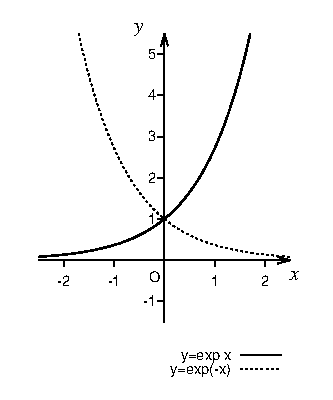
\includegraphics[width=6.0cm]{exp.eps}
    \caption{$y=\exp x$と$y=\exp(-x)$のグラフ}\label{fig:y_expx}
\end{figure}

\begin{q}\label{q:exp_graph1} 以下の関数のグラフを描け。
\begin{edaenumerate}
\item $y=1-e^{-x}$
\item $y=2(1-e^{-3x})$
\end{edaenumerate}\end{q}
\mv

さて, 指数関数を含む関数の微分を学ぼう。

\begin{exmpl} $f(x)=e^{-2x}$を微分してみよう。これを$e^y$と$y=-2x$の
合成関数と見れば(合成関数の微分を忘れた人は\pref{eq:diff_form4}へ!), 
\eref{eq:exp_diff}に注意して, 
\begin{eqnarray}f'(x)=e^{-2x}(-2x)'=-2e^{-2x}\end{eqnarray}
\end{exmpl}

\begin{exmpl} $f(x)=xe^{-2x}$を微分してみよう。まずこれを$x$と$e^{-2x}$の
積とみなして, 積の微分の公式(\pref{eq:diff_form3})より, 
\begin{eqnarray}f'(x)=e^{-2x}+x(e^{-2x})'\end{eqnarray}
右辺第二項の中の$(e^{-2x})'$は, 上の例より$-2e^{-2x}$となる。これらを組み合わせて, 
\begin{eqnarray}f'(x)=e^{-2x}-2xe^{-2x}=(1-2x)e^{-2x}\end{eqnarray}
\end{exmpl}

\begin{exmpl} $f(x)=e^{-a/x}$を微分してみよう($a$は定数)。これを$e^y$と$y=-a/x$の合成関数と見れば, 
\begin{eqnarray}f'(x)=e^{-a/x}\Bigl(-\frac{a}{x}\Bigr)'
=e^{-a/x}\Bigl(\frac{a}{x^2}\Bigr)=\frac{ae^{-a/x}}{x^2}\nonumber\\\end{eqnarray}
(例おわり)\end{exmpl}
\mv

\begin{q}\label{q:exp_diff0} 次の関数を微分せよ。
\begin{edaenumerate}
\item $f(x)=e^x$
\item $f(x)=e^{2x}$
\item $f(x)=\exp(-x^2)$
\item $f(x)=x \exp(-x^2)$
\end{edaenumerate}\end{q}
\mv


\section{対数}

第1章で学んだが, 正の実数$a, x$について($a\neq1$), 「$a$を何乗すると$x$になるか」
の指数を求める操作を, 
\begin{eqnarray}
\log_a x\label{eq:taisuu00_again}
\end{eqnarray}
とあらわす。これが対数の定義だった。ここで$a$にあたる数を\underline{底} \index{てい@底}, の$x$にあたる数を\underline{真数} \index{しんすう@真数}と呼ぶのだった。

この定義より, 
\begin{eqnarray}
\log_a x=y\label{eq:log1}
\end{eqnarray}
とは, 
\begin{eqnarray}
x=a^y\label{eq:log2}
\end{eqnarray}
と同じことである。\eref{eq:log1}を使って, \eref{eq:log2}右辺の$y$を$\log_a x$で置き換えられる。すると, 
\begin{eqnarray}
x=a^{\log_a x}\label{eq:log3}
\end{eqnarray}
となる。\eref{eq:log3}は対数の定義の言い換えにすぎないのだが, これが「わからない」
人が意外に多い。落ち着いて考えよう。$\log_a x$は, 「$a$を何乗すると
$x$になるか」である。\eref{eq:log3}の右辺は, その数で$a$を実際に「何乗かする」ことを意味
する。その結果が$x$になる(\eref{eq:log3}の左辺になる)のは当然である。\mv

注意: 対数を考える時は, 通常, 底と真数は正の実数とする。それらが負の状況は, 話が不必要にややこしくなるからである。例えば, 無理矢理に$\log_{-2}(-8)$を考えれば, それは3だろう($(-2)^3=-8$だから)。しかし, $\log_{2}(-8)$とか, $\log_{-2}8$は? と聞かれると困ってしまう。また, 通常, $1$は底として認めない。例えば$\log_{1}2$は? と聞かれると困ってしまうからだ。\mv

\begin{q}\label{q:exp_log0} $a$, $b$, $c$を正の実数として, 以下を示せ。
ただし$a \neq 1$とし, また, (8), (9)では$b \neq 1$とし, (10)では$c\neq 1$とする。
\begin{eqnarray}
&&\text{(1)}\,\,\,a^{\log_{a}b}=b\label{eq:apowlogab}\\
&&\text{(2)}\,\,\,\log_{a}a=1\\
&&\text{(3)}\,\,\,\log_{a}1=0\\
&&\text{(4)}\,\,\,\log_{a}b+\log_{a}c=\log_{a}bc\\
&&\text{(5)}\,\,\,\log_{a}\Bigl(\frac{1}{b}\Bigr)=-\log_{a}b\\
&&\text{(6)}\,\,\,\log_{a}\Bigl(\frac{b}{c}\Bigr)=\log_{a}b-\log_{a}c\label{eq:exp_log_formula6}\\
&&\text{(7)}\,\,\,\log_{a}b^c=c\log_{a}b\label{eq:log_power}\\
&&\text{(8)}\,\,\,\log_{a}b\times\log_{b}c=\log_{a}c\label{eq:logloglog}\\
&&\text{(9)}\,\,\,\log_{a}b=\frac{1}{\log_{b}a}\\
&&\text{(10)}\,\,\,\log_{a}b=\frac{\log_c b}{\log_c a}\label{eq:log_base_change}
\end{eqnarray}\end{q}
\hv

\eref{eq:log_base_change}は, \underline{底の変換公式} \index{ていのへんかんこうしき@底の変換公式}と呼ばれる。
これを使えば, どのような底の対数も, 特定の数を底とする対数の計算に変換できる。これは, 
電卓や計算機等による対数計算にしばしば有用である。\hv

\begin{exmpl} $\log_3 5$を関数電卓で求めてみよう。関数電卓の多くは, 
対数といえば常用対数や自然対数しか計算できないので, 底が3である$\log_3 5$は
直接は計算できない(ことが多い)。そこで, 底の変換公式を使って, 
$\log_3 5=\frac{\ln 5}{\ln 3}$としてやる。$\ln 5=1.609\cdots$や$\ln 3=1.098\cdots$
は関数電卓で計算できる。従って, 
\begin{eqnarray}
\log_3 5=\frac{\ln 5}{\ln 3}=\frac{1.609\cdots}{1.098\cdots}=1.464\cdots
\end{eqnarray}
と求まる。これを常用対数でやっても同じ結果になる: 
\begin{eqnarray}
\log_3 5=\frac{\log_{10} 5}{\log_{10} 3}=\frac{0.698\cdots}{0.477\cdots}=1.464\cdots
\end{eqnarray}
\end{exmpl}
\mv

\begin{q}\label{q:exp_logvalue} 以下を関数電卓で有効数字4桁で求めよ。
\begin{edaenumerate}
\item $\log_2 7$
\item $\log_{0.3} 5$
\end{edaenumerate}
\end{q}
\mv

\begin{q}\label{q:exp_log_ln} $x$を任意の正の実数とする。次式を示せ:
\begin{eqnarray}
&&\log_{10} x=(\log_{10} e)\times(\ln x)\fallingdotseq0.4343\ln x\label{eq:log2ln}\\
&&\ln x=(\ln 10)\times(\log_{10} x)\fallingdotseq2.3026\log_{10} x\label{eq:ln2log}
\end{eqnarray}\end{q}
\mv

世の中では, 対数といえば, 常用対数と自然対数がよく使われるので, 常用対数を
自然対数で表したり, その逆をしたり, というために, \eref{eq:logloglog}や
\eref{eq:log_base_change}がよく使われる。特に, ここで出てきた
\begin{eqnarray}
&&\log_{10} e\fallingdotseq0.4343\label{eq:log10e}\\
&&\ln 10\fallingdotseq2.3026\label{eq:ln10}
\end{eqnarray}
という2つの定数はよく現れる。

\begin{q}\label{q:log10e_ln10} 
\begin{enumerate}
\item \eref{eq:log10e}と\eref{eq:ln10}をそれぞれ5回書いて記憶せよ。
\item \eref{eq:log10e}と\eref{eq:ln10}の積が1になることを関数電卓を用いて確認せよ
\item それを数学的に証明せよ。
\end{enumerate}
\end{q}
\mv

ところで, $f(x)=e^x$と, $g(x)=\ln x$は, 互いに逆関数である。これは対数の定義から
明らかである。実際, 
\begin{eqnarray*}g(f(x))=\ln e^x=\log_e e^x=x\log_e e=x\end{eqnarray*}
となるし, 
\begin{eqnarray*}f(g(x))=\exp(\ln x)=e^{\log_e x}=x\end{eqnarray*}
となる(\eref{eq:apowlogab}より)。これはP.\pageref{eq:generaleq}の\eref{eq:generaleq}と整合的である。
図\ref{exp_log.eps}で明らかなように, $y=e^x$と$y=\ln x$のグラフは直線$y=x$
に関して互いに対称である(逆関数の性質。\pref{fig:func_revfunc}参照)。

\begin{figure}[h]
    \centering
    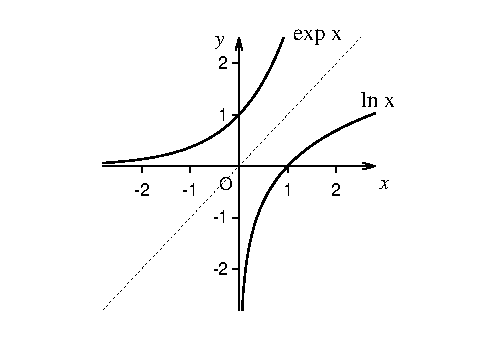
\includegraphics[width=7cm]{exp_log.eps}
    \caption{$y=e^x$と$y=\ln x$のグラフ。点線は, $y=x$のグラフ。}\label{exp_log.eps}
\end{figure}

ここで, $y=\ln x$のグラフは$0<x$の範囲でしか描かれていないことに注意。
つまり, $\ln x$という関数は, $x\le 0$では定義されない(考えることができない)
のだ。これは直感的にも明らかで, 例えば$\ln (-5)$は何か? などと言われても, 
$e=2.718\cdots$は, 何乗しようが必ず正の値であって, $-5$のような負の値は, とりようがない。

\begin{q}\label{q:exp_loggraph} 以下の関数のグラフを重ねて描け.
\begin{edaenumerate}<3>
\item $y=\log_{2}x$
\item $y=\ln x$
\item $y=\ln (1+x)$
\end{edaenumerate}\end{q}
\mv

次に, 対数関数の微分を考えよう。$f(x)=e^x$と$g(x)=\ln x$は互いに逆関数
であり, かつ, $f'(x)=f(x)$なので, 逆関数の微分(微分の公式5; \pref{eq:diff_form5})
により,
\begin{eqnarray}
(\ln x)'=g'(x)=\frac{1}{f'(g(x))}=\frac{1}{f(g(x))}=\frac{1}{x}
\label{eq:logdif}
\end{eqnarray}
である(ただし$0<x$とする)。つまり, \textgt{$\ln x$の微分は$1/x$になる}。このことは記憶せよ。
\mv

\begin{q}\label{q:exp_logdif_num} パソコンの表計算ソフトを使って, 
$\ln x$を数値微分せよ($0<x$とする)。その結果を, もとの関数($\ln x$)と, 解析的な
微分結果($1/x$)とともに, 重ねてグラフに描け。ヒント: $x=0$や$x<0$の
値では$\ln x$の計算がエラーになるので, 微妙に0より大きい$x$から始めよう。
結果は\fref{fig:difflnx}のようになるはず。
\end{q}
\begin{figure}[h]
    \centering
    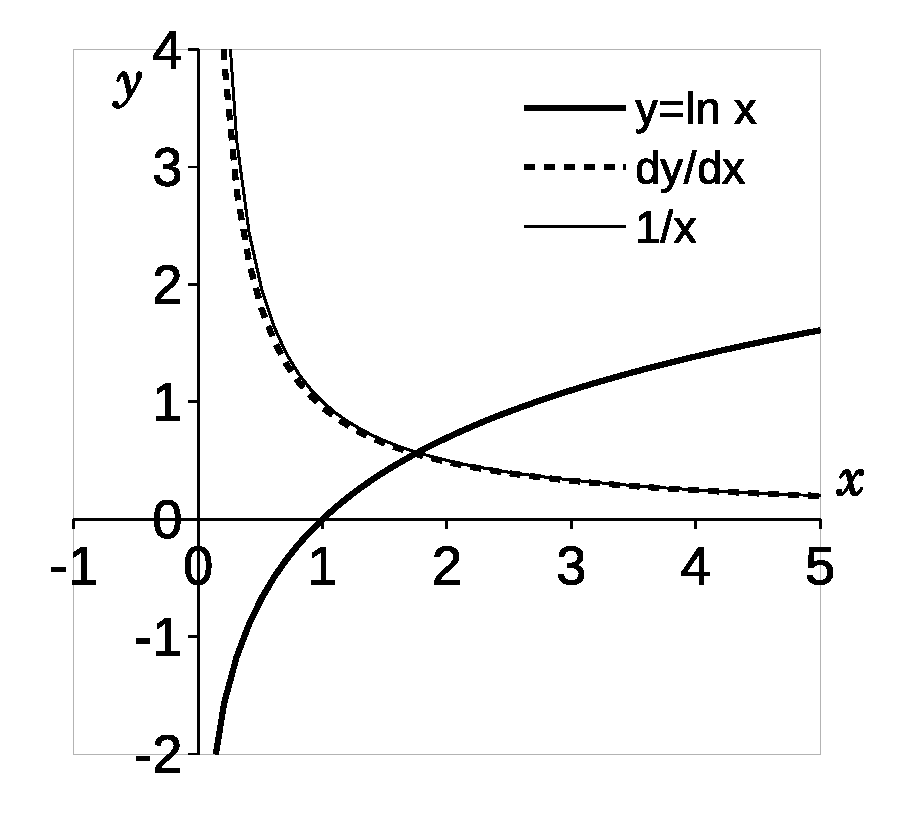
\includegraphics[width=6.5cm]{difflnx.eps}
    \caption{$y=\ln x$ (太い実線)とその数値微分(点線)のグラフ。
細い実線は$y=1/x$。$x$は0.05くらいから始めて, 刻みは0.1くらいにするときれいに描ける。}\label{fig:difflnx}
\end{figure}
\mv

\begin{q}\label{q:exp_logdif0} 以下の関数をそれぞれ微分せよ:
\begin{enumerate}
\item $\ln (x+1)$ ただし$-1<x$とする。
\item $\ln 2x$ ただし$0<x$とする。
\item $\ln |x|$ ただし$x\neq 0$とする。
\item $\ln (x-1)$ ただし$x<1$とする。
\item $\ln (1-x)$ ただし$x<1$とする。
\item $\ln |1-x|$ ただし$x\neq 1$とする。
\item \begin{eqnarray*}\ln \Bigl|\frac{x-1}{x+1}\Bigr|\quad\text{ただし}x\neq-1\text{かつ}x\neq 1\text{とする。}\end{eqnarray*}
\item $\log_{10} x$ ただし$0<x$とする。
\end{enumerate}
{\small
ヒント: (3)は$x<0$と$0<x$で場合分け。(6)は, $x<1$と$1<x$で場合分け。(7)は, いきなり合成関数の微分公式で処理するよりも, \eref{eq:exp_log_formula6}を使って変形すると楽。\\
注: これらの問題は, 「なんかややこしくてうざいな」と思うかもしれないが, 後で「積分」を学ぶときに重要な意味を持つ。また, (7)は, 生物の個体群変動を解析する理論で出てくる。}
\end{q}

\begin{faq}\small{\textgt{この問の(3)で, $\ln |x|$を微分すると$1/x$になってしまい, 絶対値が消えてしまいました。不思議です。} ... 場合分けしたのに, 結果は一緒って奇妙ですよね。図\ref{fig:difflnx}を使って考えてみましょう。$\ln |x|$のグラフは, この図を$y$軸でひっくり返して, 左右対称にしたものです。$y$軸の左側($x<0$)では, 左から$x=0$に近づくにつれて, $\ln |x|$は「奈落の底」に落ちていきます。つまり, 傾き(つまり$(\ln x)'$)はマイナス。といっても, $x=0$のはるか左では, 傾きはきつくないので, $(\ln x)'$はほぼ0。しかし, $x=0$に近づけば近づくほど傾きは急になるので, $(\ln x)'$の値はどんどん小さくなる(負の大きい値になる)。それはちょうど, $1/x$のグラフの, $x<0$での挙動によく似ている(というか一緒)です。}\end{faq}
\mv




\section{対数微分}

関数$f(x)=a^x$を微分してみよう(ただし$a$は1以外の正の定数とする)。このままではこの関数は微分できそうにない。そこで, まず, $f(x)=a^x$の両辺の
対数をとると, 
\begin{eqnarray}\ln f(x)=x\ln a\end{eqnarray}
ここで両辺を微分する。左辺の微分は, 合成関数の微分の公式から, 
\begin{eqnarray}\{\ln f(x)\}'=\frac{f'(x)}{f(x)}\end{eqnarray}
右辺の微分は, $\ln a$である。従って, 
\begin{eqnarray}\frac{f'(x)}{f(x)}=\ln a\end{eqnarray}
従って, 
\begin{eqnarray}f'(x)=(\ln a)f(x)=(\ln a)\,a^x\label{eq_diff_ax}\end{eqnarray}
となる。このように, 両辺の対数をとってから微分
するテクニックを\underline{対数微分} \index{たいすうびぶん@対数微分}という。\hv

\begin{q}\label{q:exp_diffxpowx} 対数微分を使って, 次式を示せ:
\begin{eqnarray}\frac{d}{dx}x^x=(1+\ln x)\,x^x\label{eq_diff_xx}\end{eqnarray}
ヒント: $f(x)=x^x$と置き, 両辺の$\ln$をとって, それらを$x$で微分。$x\ln x$の微分は
積の微分の公式を使う。
\end{q}

ちなみに, 問\ref{q:exp_diffxpowx}で考えた関数$x^x$のグラフは, 図\ref{fig:x_pow_x}
のようになる。これを見ると, \eref{eq_diff_xx}が0になるとき, つまり$x=1/e$で
最小値をとることがわかる。
\begin{figure}[h]
    \centering
    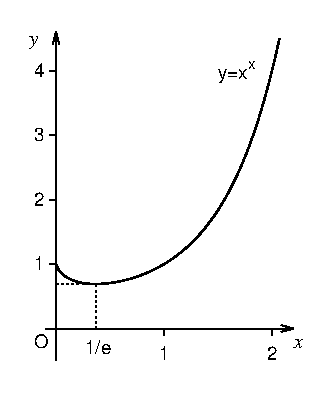
\includegraphics[width=4.5cm]{x_pow_x.eps}
    \caption{$y=x^x$のグラフ。}\label{fig:x_pow_x}
\end{figure}

\begin{freqmiss}{\small\textgt{$x^x$の微分を, 「$(x^{\alpha})'=\alpha x^{\alpha-1}$」という
公式(P.\pageref{eq:diff_form6}の\eref{eq:diff_form6})に「当てはめ」て, $(x^{x})'=x x^{x-1}=x^x$
としてしまう} ... $(x^{\alpha})'=\alpha x^{\alpha-1}$は, $\alpha$が定数の
ときにしか成り立ちません。この間違いでは, 指数部分の$x$を$\alpha$に見立てて
しまっていますが, $x$は定数ではないので, このような適用は許されません。
それに, $x=1/e$でこのグラフの傾きは0になっているので, そこでの微分係数は0
のはず。でも, $x^x$に$x=1/e$を入れたら, $(1/e)^{1/e}=0.692\cdots$で, 0に
なりません。だから, 少なくとも$x=1/e$では$(x^x)'=x^x$は成り立ちません。}\end{freqmiss}
\mv





\section{ガウス関数}\index{がうすかんすう@ガウス関数}
$a$を正の定数として, 
\begin{eqnarray}
f(x)=\exp(-ax^2)\label{eq:Gauss_func}
\end{eqnarray}
という形の関数を\underline{ガウス関数} (Gauss function)という。ガウス関数は, 統計学をはじめ, 様々な分野で
重要な関数なので, ここでいくつか性質を調べておこう。\mv

\begin{q}\label{q:exp_Gauss} ガウス関数に関して, 以下のことを示せ:
\begin{enumerate}
\item 偶関数である。
\item 常に0より大きい。
\item $f'(0)=0$である(だから$x=0$での接線は水平)。
\item $x$が大きくなると, 0に近づいていく。
\item $x=0$で最大値をとる。
\end{enumerate}\end{q}\mv

これらから, ガウス関数のグラフは, $x=0$を頂点とする, 左右対称の山形のグラフになることが
想像できる。\mv

\begin{q}\label{q:exp_Gauss_graph} 以上のことから, 
\begin{enumerate}
\item $a=1$のときのガウス関数のグラフを描け。
\item $a$が1より大きくなるとグラフはどう変わるか? 
\end{enumerate}\end{q}

\begin{figure}[h]
    \centering
    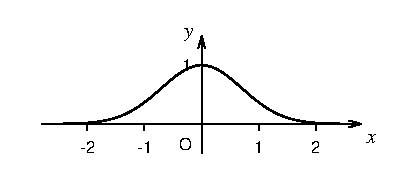
\includegraphics[width=7cm]{Gauss_fnc.eps}
    \caption{ガウス関数$y=\exp(-x^2)$のグラフ。常に$y>0$なので, 
本当は$x$軸と重なることは無いのだが, $x$がある程度大きくなると, 
非常に速く$x$軸に接近するので, $|x|$が3や4くらいになったら
$x$軸にぴったり重ねて描いてもかまわない(むしろその方が実情に近い)。
\label{fig:Gauss_func}}
\end{figure}

\begin{freqmiss}{\small\textgt{$y=\exp(-x^2)$のグラフを, $y=e^{-x}$のような左右非対称
なグラフを描いたり, 最大値のところで尖ったグラフを描いてしまう。} ... 偶関数のグラフは左右対称でしょ?}\end{freqmiss}
\mv


\section{対数グラフ}\index{たいすうぐらふ@対数グラフ}

実験データの解析等で, 軸が対数で目盛られたグラフをよく使う。図\ref{fig:log_graph}は, 
横軸は普通の目盛だが縦軸が対数目盛になったグラフである。このように片方の軸が
対数目盛のグラフを\underline{片対数グラフ} \index{かたたいすうぐらふ@片対数グラフ}という。
対数軸には, 以下のような特徴がある:
\begin{itemize}
\item "0"が存在しない。下に行くほど0に近づくが, 決して0をグラフ上で表現することはできない。
\item 太い目盛りをひとつ移動すれば値が10倍になる。
\item 細い目盛りをひとつ移動すれば最上位の桁の値がひとつ増える。
\end{itemize}

\begin{figure}[h]
    \centering
    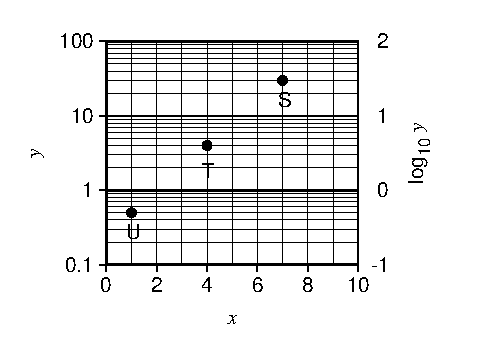
\includegraphics[width=8cm]{log_paper.eps}
    \caption{片対数グラフの例。左の軸に振られている目盛りは, 対数にする前の値の目盛り(だから変な間隔になっている; グラフ上に点を打つときは便利)。右の軸に振られている目盛りは, 対数にした後の値の目盛り。直線の傾きは右側の目盛りで求める。なお, 
世の中の多くの対数グラフでは, 左のような軸か, 右のような軸のどちらか片方だけが, 左側に書かれている。\label{fig:log_graph}}
\end{figure}

例えば図\ref{fig:log_graph}で, 点Sの値は$(7, 30)$である。
点Sよりひとつ上の細目盛り線は$y=40$の線である。点Tの値は$(4, 4)$である。

\begin{q}\label{q:exp_loglingraph0} 点Uの値を読み取れ。\end{q}\mv

このような変なグラフを使う理由は, 2つある。ひとつには, 対数目盛りを使うことで, 
非常に範囲の広い値を, ひとつのグラフにコンパクトに表現できるからである。例えば, 0.1, 1, 10, 100の4つの
データをふつうの目盛りにプロットすると, "100"だけが飛び抜けて上の方に行ってしまう一方, "0.1"と
"1"はほとんど固まってしまって見分けづらい。しかし対数目盛りにプロットすると, これらのデータは
等間隔に並ぶのだ。

もうひとつの理由は, そもそも自然界に多く存在する指数関数的な現象(細菌の増殖, 光の減衰, 
化学物質の一次反応などなど)の様子を調べるには, このグラフが好都合だというものだ。というのも, 
ある現象が, 
\begin{eqnarray}
y=Ae^{ax}\label{eq:loggraph_Aeax}
\end{eqnarray}
という関数(それは\eref{eq:diffeq0}の形の微分方程式の解だった!)であらわされることが
確実な場合, 実験データによって定数$A, a$を決定したい, ということ
がよくある。その場合, 上の式の両辺の常用対数をとると, 
\begin{eqnarray}
\log_{10} y=\log_{10} A + ax(\log_{10}e)
\end{eqnarray}
となる。この場合, $\log_{10} y$は$x$の一次関数(直線関係)になる。これを
片対数グラフにプロットすると, その傾き($a\log_{10}e$)から$a$の値がわかり, 切片(横軸の座標が0になるときの値; 
$\log_{10}A$)から$A$の値がわかるのだ。

ただし, この方法で傾きを求める時には注意が必要だ。傾きは, 縦軸方向の変化量を横軸方向の
変化量で割れば求まるが, その時, 縦軸(対数軸)方向の変化量は, 
実際の変化量(対数を取る前の$y$の変化量)でなくて, いったん対数に変換したあとの変化量
($\log_{10} y$の変化量)である。例えば図\ref{fig:log_graph}では, 点Tと点Sでは,  
実際の変化量($y$の変化量)は, 左側の軸で値を読み取って, $30-4=26$である。しかし,  
対数としての変化量($\log_{10}y$の変化量)は, 右側の軸の値で考えねばならない。
それにはまず, 点Tから点Sまでの高さを定規で計り, 一方で, 太い目盛り線の間隔
(右側の軸で1に相当する変化量; 左側の軸では「10倍」に相当する変化量)も定規で計り, 
前者を後者で割り算する。そうやって得たのが「縦軸の変化量」である。そして, 
\begin{eqnarray}
\text{傾き}=\frac{\text{縦軸の変化量}}{\text{横軸の変化量}}=a\log_{10} e
\end{eqnarray}
が成り立つ。従って, 
\begin{eqnarray}
a=\frac{1}{\log_{10} e}\,\frac{\text{縦軸の変化量}}{\text{横軸の変化量}}
\fallingdotseq2.3026\,\frac{\text{縦軸の変化量}}{\text{横軸の変化量}}\nonumber\\
\label{eq:logplot_a05}
\end{eqnarray}
によって$a$の値が求まる。ちなみに, もしも\eref{eq:loggraph_Aeax}
ではなく$y=A\times10^{ax}$のような関数を想定していれば, \eref{eq:logplot_a05}
の$1/\log_{10}e$や2.3026という数は必要ない。\mv

\begin{q}\label{q:exp_loglingraph1} 図\ref{fig:log_graph}のグラフについて, 
3点S, T, Uを最もうまく結ぶようなひとつの直線を引いて, 
その傾きと切片から, $y=Ae^{ax}$の定数$A$と$a$の値を推定せよ。その際, 
定規で測定して得た数値と, それをもとに行った計算式も明記せよ。また, 
推定された$A$と$a$の値を用いて, 3つの点S, T, Uは, うまく再現されるか? \end{q}\mv

図\ref{fig:log_log_graph}は, 横軸と縦軸が対数目盛になったグラフ用紙である。このようなグラフを\underline{両対数グラフ}
\index{りょうたいすうぐらふ@両対数グラフ}という。

\begin{figure}[h]
    \centering
    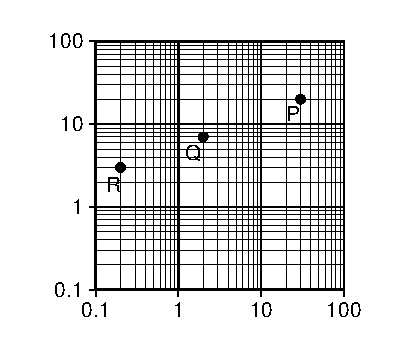
\includegraphics[width=8cm]{log_log_paper.eps}
    \caption{両対数グラフの例。\label{fig:log_log_graph}}  
\end{figure}

例えばこのグラフで, 点Pの座標は$(30, 20)$である。\mv

\begin{q}\label{q:exp_logloggraph0} 点Qと点Rの座標をそれぞれ読み取れ。\end{q}\mv


両対数グラフを使う理由は, まず, 片対数グラフと同様に, 非常に範囲の広い値を, ひとつのグラフ
にコンパクトに表現するためである。

もうひとつの理由は, 指数関数に劣らぬくらいに自然界に多く存在する, べき関数的な現象
\footnote{例えば, 本川達雄「ゾウの時間 ネズミの時間」(中公新書)参照。ある種の
現象がべき関数で表現できることを, power lawとかscalingと呼ぶ。powerとは「べき」のこと。}
を調べるには, このグラフが好都合だというものだ。というのも, ある現象が, 
\begin{eqnarray}
y=Ax^a\label{eq:exponential_power00}
\end{eqnarray}
という関数(べき関数)\index{べきかんすう@べき関数}であらわされる場合, 実験データによって定数$A, a$を決定したい, 
ということがよくある。その場合, \eref{eq:exponential_power00}の両辺の常用対数をとると, 
\begin{eqnarray}
\log_{10} y=\log_{10} A + a \log_{10} x\label{eq:exponential_power02}
\end{eqnarray}
となる。従って, もし現象がべき関数的であるならば, そのデータを両対数グラフにプロットすると, 
直線になり, その直線の傾き(適当な2点の間の, グラフ用紙上での横の距離と縦の距離を定規で測って, 
後者を前者で割ればよい)が$a$の値であり, 切片($\log_{10} x=0$となるときの$y$座標の値)が
$A$の値なのだ\footnote{片対数グラフのときと違って, 両対数グラフは, 底が$e$のときも
$10$のときも, 直線の傾きはかわらない。}。\mv

\begin{q}\label{q:exp_logloggraph1} 図\ref{fig:log_log_graph}のグラフについて, 
3つの点P, Q, Rを最もうまく結ぶようなひとつの直線を引いて, 
その傾きと切片から, $y=Ax^a$の定数$A$と$a$の値を推定せよ。
その際, 定規で測定して得た数値と, それをもとに行った計算式も明記せよ。また, 
推定された$A$と$a$の値を用いて, 3つの点P, Q, Rは, うまく再現されるか?\end{q}
\mv


%\begin{q}\label{q:exp_English} 指数・対数に関する以下の言葉を英訳せよ:
%\begin{edaenumerate}
%\item エクスポーネンシャル
%\item 対数
%\item 底(対数の)
%\end{edaenumerate}
%\end{q}\mv



\section{指数関数の微分方程式}\label{sect_diffeq_exp}

ところで, 唐突ではあるが, 
\begin{eqnarray}
\frac{d}{dx}f(x)=3f(x)\label{eq:exp_diffeq_sol00}
\end{eqnarray}
という式を考えよう。
この\eref{eq:exp_diffeq_sol00}は, 関数$f(x)$に関する方程式
とみなすことができる。一般に, 関数に関する方程式で, なおかつ
その関数の微分を含むような方程式を\underline{微分方程式}
\index{びぶんほうていしき@微分方程式}という。\eref{eq:exp_diffeq_sol00}
は一種の微分方程式である。

第\ref{chapt:algebra}章で学んだ代数方程式は, $x$などで表される
「数」に関する方程式だった。つまり, その「解」は数値である。一方, 
微分方程式は, $f(x)$などで表される「関数」に関する方程式である。
つまりその「解」は関数である。

さて, 例えば関数「$f(x)=x^2$」は, \eref{eq:exp_diffeq_sol00}の解だろうか? 
\eref{eq:exp_diffeq_sol00}の左辺にこの関数を代入すると, 
$\frac{d}{dx}x^2=2x$となるが, 右辺にこの関数を代入すると, 
$3x^2$となる。$2x=3x^2$は恒等的には成り立たない($x=1$や$x=2$の
ときは成り立たない)。従って, 関数「$f(x)=x^2$」は, \eref{eq:exp_diffeq_sol00}の解
ではない!

\begin{q}\label{q:exp_diffeq_sol00} 
以下の関数が, \eref{eq:exp_diffeq_sol00}の解であるかどうかを調べよ。
注: (5)(6)は定数関数。
\begin{edaenumerate}<3>
\item $2x$
\item $2e^{3x}$
\item $3e^{2x}$
\item $-5e^{3x}$
\item $2$
\item $0$
\end{edaenumerate}
\end{q}

ここでわかったように, ひとつの微分方程式には, 複数の解がありえるのだ。\\

ここでは証明しないが, \eref{eq:exp_diffeq_sol00}の解は, 
「定数×$e^{3x}$」という形の関数である, ということがわかっている。もっと一般的に言えば, 以下の
ような定理が知られている:
\begin{itembox}{定理}
$\alpha$を0でない定数として, 
\begin{eqnarray}
\frac{d}{dx}f(x)=\alpha f(x)\label{eq:diffeq0}
\end{eqnarray}
という微分方程式の解(その方程式を恒等的に成り立たせるような関数)は, 
\begin{eqnarray}
f(x)=\beta e^{\alpha x}\label{eq:diffeq000}
\end{eqnarray}
という関数である($\beta$は任意の定数)。
\end{itembox}

\begin{q}\label{q:exp_diffeq_sol20} \eref{eq:diffeq000}は
\eref{eq:diffeq0}の解であることを示せ。\end{q}

\begin{faq}\small{\textgt{\eref{eq:diffeq0}の解は\eref{eq:diffeq000}
のような形の関数の他にはありえないのですか?} ... その理由はまだ説明できません
(いずれ説明します)が, ありえません。とりあえず今は, \eref{eq:diffeq0}
の形の微分方程式の例をいくつか経験して慣れてください。}\end{faq}
\mv

\eref{eq:exp_diffeq_sol00}は, \eref{eq:diffeq0}で$\alpha=3$とした
ケースだったのだ。その解が複数あったのは, \eref{eq:diffeq000}で
$\beta$の値が何でもよかったからなのだ。\\

さて, $\beta$はどんな値でもよいのだが, $\eref{eq:diffeq000}$で$x=0$と置くと, 
\begin{eqnarray}
f(0)=\beta e^{0}=\beta\label{eq:diffeq000_IC0}
\end{eqnarray}
となる。つまり, $\beta=f(0)$と表すことができる。これを\eref{eq:diffeq000}に
入れると, 
\begin{eqnarray}
f(x)=f(0)e^{\alpha x}\label{eq:diffeq000_IC}
\end{eqnarray}
となる。生物資源学類生にとって大事なことは, 「\eref{eq:diffeq0}の形の
微分方程式の解は\eref{eq:diffeq000_IC}である」ということだ。なぜなら, 
この形の微分方程式が, 生物資源学類の(数学以外の)様々な授業や
実験、研究でガンガン出てくるからである。\\



\section{放射性核種(放射能)の崩壊}\label{sect:func_radioactive}

ここからは, 指数・対数の応用例の話である。

炭素には, 原子量12の普通の炭素原子の他に, 原子量13の炭素原子と原子量14の炭素原子がある。一般に, 
同じ元素(ここでは炭素)なのに互いに原子量が違う原子のことを, 「同位体」(isotope)と呼ぶ。このうち, 
原子量13の炭素同位体($^{13}$C)は原子核崩壊しないが, 原子量14の炭素同位体($^{14}$C)は徐々に原子核崩壊\footnote{この場合は, 放射線(ベータ線: 高速の電子線)を出しながら崩壊する
「ベータ崩壊」\index{べーたほうかい@ベータ崩壊}。}をして, 原子量14の窒素原子($^{14}$N)
に変わってしまう。この崩壊の様子を数学的に考えてみよう。

$^{14}$Cの個数を, 時刻$t$の関数$C(t)$で表すことにしよう。
いま, 時刻$0$年で$C_0$モルの$^{14}$Cがあるとする(つまり, $C_0:=C(0)$)。
これがどんどん崩壊して減っていくのだが, 
時刻$t$年目のとき$C(t)$モルであるとして, $t$年目から$t+dt$年目の間(ごく短い時間を考える)に, 
その一部が放射性崩壊して別の元素(窒素)に壊変する。その変化は, まず, そのときの個数$C(t)$に
比例する。これは常識的に明らかで, 母数(崩壊するもとの原子の数)が倍になれば, 一定時間内の
崩壊回数も倍になる, というだけの話である。また, 時間間隔$dt$にも比例する。これも, 時間が長いほど
崩壊もたくさん起きるだろうという常識的な判断による。ただし, $dt$が長すぎると, その間にも母数
$C(t)$がどんどん減ってくるので, この判断は成り立たない。あくまで, $dt$が十分に短いことを想定した
判断である。以上の考察から, 
\begin{eqnarray}
C(t+dt)=C(t)-\alpha C(t) dt
\end{eqnarray}
と書ける。$\alpha$はなんらかの定数である($0<\alpha$とする)。$C(t)$は減る方向なので, 
右辺第二項の符号はマイナスである。この式を変形すれば, 
\begin{eqnarray}C(t+dt)-C(t)=-\alpha C(t) dt\label{eq:dC_dt_4}\end{eqnarray}
両辺を$dt$で割ると, 
\begin{eqnarray}\frac{C(t+dt)-C(t)}{dt}=-\alpha C(t)\end{eqnarray}
ここで$dt$が十分に小さいことを考えると, 左辺は$C(t)$の微分(導関数)である。従って次式を得る:
\begin{eqnarray}
\frac{dC}{dt}=-\alpha C(t)\label{eq:C14disint1}
\end{eqnarray}
これが, 放射性炭素の崩壊に関する微分方程式である。\\

\eref{eq:C14disint1}は, $C$を$f$, $t$を$x$, $-\alpha$を$\alpha$に読み替えると, \eref{eq:diffeq0}
になる。従って, \eref{eq:C14disint1}の解は, \eref{eq:diffeq000_IC}のようになるはずだから, 
\begin{eqnarray}
C(t)=C_0\,e^{-\alpha t}\label{eq:C14disint3}
\end{eqnarray}
となる。従って, $C_0$, つまり$t=0$(つまり最初)のときの$C$の値がわかれば, 
\eref{eq:C14disint3}によって, その後の$C$がどのように変化するかが, 
予測できるのである。\\

\begin{q}\label{q:C14disint} 放射性炭素の崩壊が\eref{eq:C14disint3}
のように予測できることを説明せよ(上の議論を簡潔にまとめればOK)。\end{q}

ところで, 放射性炭素の問題に戻ると, 通常は, \eref{eq:C14disint3}のかわりに, 
次のような式がよく使われる: 
\begin{eqnarray}
C(t)=C_0\Bigl(\frac{1}{2}\Bigr)^{\frac{t}{t_h}}\label{eq:C14disint5}
\end{eqnarray}
$t_h$は「半減期」\index{はんげんき@半減期}と呼ばれる定数であり, $^{14}$Cの場合,
\begin{eqnarray}
t_h=5730\text{年}\label{eq:C14halfyear}
\end{eqnarray}
であることが知られている。
\vv

\begin{q}\label{q:funct_52} \eref{eq:C14disint5}について, 
\begin{enumerate}
\item \eref{eq:C14disint5}を, 横軸$t$, 縦軸$C(t)$のグラフにかけ。
\item $C(t_h)$はもとの値$C_0$の半分であることを確かめよ。この故に, $t_h$を半減期と呼ぶ。
\item \eref{eq:C14disint5}を, \eref{eq:C14disint3}の形に変形せよ。ヒント: $1/2=\exp(-\ln 2)$
\item 半減期は, \eref{eq:C14disint3}の定数$\alpha$とどのような関係にあるか?
\item 式(\ref{eq:C14halfyear})から, 定数$\alpha$の値を求めよ。
\end{enumerate}\end{q}
\vv

上で, $C_0$がわかればその先のことが予測ができると書いたが, 実際にこの式を
使う場面では, むしろ, 「$C_0$だけでなく現在の値$C(t)$もわかっているが, 
$t$がわからない」という状況の方が多い。それは, 次のような状況である: 
生物体は, 生きている間は
大気のCO$_2$の中の$^{14}$Cと同じ比率の$^{14}$Cを持っているが, 
死ぬと地球大気との交換が止まるので, $^{14}$Cがだんだん減って行く。一方, 地球大気の$^{14}$Cは, 
宇宙線によって生産されるのと崩壊するのがつりあって, 常にほとんど一定の比率をしていることが
わかっている(それが$C_0$に相当する)。これらのことから, 昔に生きていた
生物体の遺骸の現在の$^{14}$Cの比率を調べることで, その生物が生きていた
年代を推定するのだ\footnote{
生物遺骸の年代推定は, 防災科学において重要な情報を与えてくれる。例えば, 
過去の火山噴火や津波等によって形成された堆積物の層の中に, 
木片などの生物遺骸を見つけることができれば, その年代を測ることで, 
その火山噴火や津波の起きた時期を知ることができる。そのような情報があれば, 
その地域で将来的に起こりうる災害の規模や頻度を想定することができ, 
それをもとに災害対策を立てることができる。}。
\hv

\begin{q}\label{q:funct_54} 昔の火山噴火によってできた火山灰の地層の
中から木の枝が出てきた。その木の枝の$^{14}$Cの比率は, $C_0$の1/4であった。
その木が埋まって死んだ年代, つまり火山噴火の起きた年代はいつごろか?\end{q}
\hv 


\section{化学反応速度論}\label{sect:func_chemreact}

前節で考えたのと似たような話が, 生物資源学類の「化学」や「化学実験」で出てくる。
それは「化学反応速度論」だ。いろんな化学反応がどのくらい速く進むかを考える
理論だ。ここでは単純に, 一種類の化学物質Aが, 別の化学物質Bと化学物質Cに
分解するような場合:
\begin{eqnarray}\mbox{A} \longrightarrow \mbox{B}+\mbox{C}\label{eq:chem_react1}\end{eqnarray}
の化学反応速度論を学ぼう。ただし反応は左から右に一方向にしか進まないとする。

Aの量(モル濃度)を[A]と書く。[A]は時刻$t$の関数なので, [A]$(t)$と書くべきだが, 煩雑なので, 
基本的に「$(t)$」は省略する。$dt$を微小な時間間隔とする。この$dt$の間にAからB+Cに変化する
反応の回数を考える: まず, 物質Aの全体の中のある割合が物質Bと物質Cに変わると考えられるから, 
反応の回数は, Aの現存量, つまり[A]に比例するだろう(量が2倍になれば, 反応する回数も2倍に
なるだろう!)。そして, これは時間間隔$dt$にも比例するだろう(目の前で1秒間に10回の反応が
起きているなら, 2秒間では20回の反応が起きるだろう!)。つまり, この回数は, ある正の定数$k$を用いて, 
\begin{eqnarray}
k\mbox{[A]}\,dt\label{eq:chem_react12}
\end{eqnarray}
と書けるはず。この回数のぶんだけ, [A]は減るわけだ。従って, $dt$の間の[A]の変化量
$d\mbox{[A]}$は\footnote{$d\mbox{[A]}=\mbox{[A]}(t+dt)-\mbox{[A]}(t)$である。}, 
\begin{eqnarray}
d\mbox{[A]}=-k\mbox{[A]}dt\label{eq:chem_react13}
\end{eqnarray}
となる。すなわち, [A]は, 
\begin{eqnarray}
\frac{d\mbox{[A]}}{dt}=-k\mbox{[A]}\label{eq:diffeq_1_chem_react}
\end{eqnarray}
という微分方程式を満たすはず\footnote{\eref{eq:chem_react13}から\eref{eq:diffeq_1_chem_react}
への式変形を詳しく書くとこうなる:
\begin{eqnarray*}
&&\mbox{[A]}(t+dt)-\mbox{[A]}(t)=-k\mbox{[A]}dt\\
&&\frac{\mbox{[A]}(t+dt)-\mbox{[A]}(t)}{dt}=-k\mbox{[A]}\\
&&\frac{d\mbox{[A]}}{dt}=-k\mbox{[A]}
\end{eqnarray*}
}。ここで右辺にマイナスがついたのは, [A]が「減る」ことを表す。
\eref{eq:diffeq_1_chem_react}の左辺は, [A]の変化の速さ, すなわち「反応速度」
を意味する。\eref{eq:diffeq_1_chem_react}のように, 反応速度が物質量の一次式
で表現できるような化学反応を「1次反応」という。$k$は「反応速度定数」\index{はんのうそくどていすう@反応速度定数}
と呼ばれ, 主に反応の種類と温度, 触媒の有無等によって決まる。詳しくは生物資源学類の
「化学I」の講義で習おう!\\

\eref{eq:diffeq_1_chem_react}は, [A]を$f$, $t$を$x$, $-k$を$\alpha$に読み替えると, \eref{eq:diffeq0}
になる。従って, \eref{eq:diffeq_1_chem_react}の解は, \eref{eq:diffeq000_IC}のようになるはずだから, 
\begin{eqnarray}
\mbox{[A]}(t)=\mbox{[A]}(0)e^{-kt}\label{eq:chem_react7}
\end{eqnarray}
となる。[A]$(0)$は反応のスタート時点(実験開始の時点)での[A]の値
なので, 実験者はわかっているはずだ(そういうのを調べないで実験を始める
人は科学者ではない!)。従って, \eref{eq:chem_react7}によって, この反応中の
物質Aの量がどう変化するかが, 予測できるのである。\\

\begin{q}\label{q:diffeq_1_chem_react} \eref{eq:chem_react1}の
ような化学反応が\eref{eq:chem_react7}のように予測できることを説明せよ。
(上の議論を簡潔にまとめればOK)。\end{q}

生物資源学類の「化学実験」では, 実際にこのような反応の例として, 
酢酸メチルという物質の加水分解を実験し, このような数学を使って
解析する。他にも, 農地に撒かれた農薬の残留性なども, このような
数学で解析される。\\



\section{ロジスティック曲線}\label{sect:logistic_curve}

$a, b, c$を正の定数として, 
\begin{eqnarray}
f(x)=\frac{1}{a+be^{-cx}}\label{eq:logistic_func0}
\end{eqnarray}
という形の関数を, ロジスティック関数と呼ぶ。この関数は, 生物学や統計学などで
よく使う。どう使うかは先々のお楽しみにしておいて, ここではこの関数のグラフを描いてみよう。

\begin{q}\label{q:logistic_func}\eref{eq:logistic_func0}について, 
\begin{enumerate}
\item $f(0)=1/(a+b)$であることを示せ。
\item 分母, すなわち$a+be^{-cx}$は, $x$が増えるにつれて減少することを示せ。
\item $f(x)$は, $x$が増えるにつれて増加することを示せ。
\item $x\rightarrow\infty$のとき, $f(x)$はどうなるか?
\item $x\rightarrow-\infty$のとき, $f(x)$はどうなるか?
\item $f'(0)$を求めよ。
\item 以上を元に, $y=f(x)$のグラフを手で描け。結果は\fref{fig:logistic_abc}のようになる。
このグラフをロジスティック曲線と呼ぶ。\index{ロジスティックきょくせん@ロジスティック曲線}
\end{enumerate}
\end{q}

\begin{figure}[h]
    \centering
    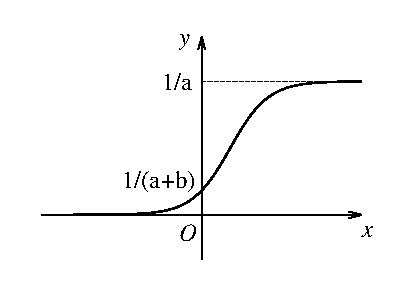
\includegraphics[width=6.0cm]{logistic_abc.eps}
    \caption{\eref{eq:logistic_func0}(ロジスティック曲線)のグラフ。$x=0$での
接線の傾きは$bc/(a+b)^2$}\label{fig:logistic_abc}
\end{figure}


特に, $a=b=1$のときは, \eref{eq:logistic_func0}はシグモイド関数\index{しぐもいどかんすう@シグモイド関数}
と呼ばれる。これは, 生物の神経細胞の性質を表すのに使われ, 
「ニューラルネット」と呼ばれる技術(いわゆる「ディープ・ラーニング」とか
「人工知能」の一部)の基礎である。\\

\begin{faq}\small{\textgt{微分→指数・対数→三角関数→積分
の順番で勉強するのはなぜですか?} ... 指数・対数・三角関数の
理解に微分が役立つので, 微分を先にやります。指数・対数・三角関数は
他の科目(物理・化学・各種実験等)で早く必要になるので, 早めにやります。
というわけで, 積分が後になりました。}\end{faq}

\begin{faq}\small{\textgt{自分は今まで何もわかっていなかったということを痛感しました。}
... 「無知の知」(ソクラテス)ってやつですね。知性の出発点です。}\end{faq}

\begin{faq}\small{\textgt{やっぱり, 分かってるつもりでも実際に問題
を解いてみると全然分かってなかったことに気づいた。}
... だから「読んで理解する」だけではダメです。}\end{faq}

\begin{faq}\small{\textgt{みんなより出来なさ過ぎて焦ります。}
... 人は人, 自分は自分。急がず焦らずこつこつやり続ければ, 必ず追いつけます。}\end{faq}

\begin{faq}\small{\textgt{質問に行ったらすごくよくわかり, すっきりしました。}
... 聞くは一時の恥, 聞かぬは一生の損。いつでもおいで。}\end{faq}
\hv

\section*{演習問題}

\begin{exq}\label{q:funct_nucl_acc} 福島第一原子力発電所の事故では, 
2011年3月15日前後に, 大量の放射性物質が放出されてしまい, 各地に降下した。
そのとき放出された放射性物質は, 徐々に崩壊して減っている。以下の放射性物質は, 
現在, 当初の何倍になったか? (有効数字2桁で)
\begin{enumerate}
\item ヨウ素131 ($^{131}$I; 半減期8.02日)
\item セシウム134 ($^{134}$Cs; 半減期2.07年)
\item セシウム137 ($^{137}$Cs; 半減期30.1年)
\end{enumerate}
{\small ヒント: \eref{eq:C14disint5}を用いて$C(t)/C(0)$を求めればよい。}
\end{exq}
\mv

\begin{exq}\label{q:funct_nucl_acc2} 君は「ベクレル」(Bq)という単位を
聞いたことがあるだろうか? これは, 放射性物質が1秒間に崩壊する個数
\footnote{崩壊するときに放射線が発せられるので, それを検知することに
よって, 崩壊する個数は比較的容易に計測できる。}を表し, 
その放射性物質がどのくらいあるかを間接的に表す指標になる。ある食品に
含まれる$^{137}$Csは, 200~Bqであった (1秒間あたり200回の崩壊を起こした)。
この食品には, 何個の$^{137}$Csが含まれているか? (有効数字2桁で) 
{\small ヒント: \eref{eq:dC_dt_4}を使う。左辺は変化した個数を表しているから, 
ここでは$-200$個。右辺の$C(t)$が未知数。$dt$=1~秒。
$\alpha$は前問で示された半減期から求める。}\end{exq}
% 2.7*10^11個。
\mv

\begin{exq}\label{exq:exp_diff_powpow}
対数微分を使わないで, 関数$a^x$と関数$x^x$をそれぞれ微分せよ($1<a$)。
ヒント: $a=e^{\ln a}$を使って, $a^x=(e^{\ln a})^x$と変形。同様に, 
$x^x=(e^{\ln x})^x$。そして指数法則, そして合成関数の微分。\end{exq}
\mv

\begin{exq}\label{exq:func_veg_cover_erosion} 森林や草原, 農地では, 植物の葉
が地表を覆うことで土壌浸食を抑制する。この効果を調べるために, 葉の量と地表面被覆率の関係を調べよう。
\begin{enumerate}
\item 1 m$^2$の地表の上に, 0.01 m$^2$(100 cm$^2$)の水平な葉が1枚あれば, 
地表面の1\%が被覆される(被覆率0.01)。では1 m$^2$の地表の上に, 1枚あたり
$p$ m$^2$の水平な葉が$n$枚, ランダムに分布するとき, 葉による地表面の被覆率
$F$は, 
\begin{eqnarray}
F=1-(1-p)^n
\end{eqnarray}
となることを示せ(葉の重なりがあることに注意せよ)。
\item 1 m$^2$の地表の上に存在する葉の総面積が一定値$L$ m$^2$であるとする。すなわち, 
\begin{eqnarray}np=L\label{eq:func_L_Poisson03}\end{eqnarray}
である。$F$を$n$と$L$であらわせ($p$を消去せよ)。
\item \eref{eq:func_L_Poisson03}の$L$が一定, という条件のもとで, 
$n \rightarrow \infty$, $p\rightarrow 0$のとき, 
\begin{eqnarray}F=1-e^{-L}\end{eqnarray}
となることを示せ。これは, 1枚1枚の葉の大きさが十分小さいと
みなせるときに, 葉が全体として地表面を覆う割合を与える理論である。
\item 1 m$^2$の地表の上にある葉の総面積が1 m$^2$のときに地表面を覆う割合は, どのくらいか?
\end{enumerate}\end{exq}
\mv

\begin{exq}\label{q:func_log_magnitude} 地震のエネルギーは, 
マグニチュード\index{まぐにちゅーど@マグニチュード}
という指標であらわされることが多い。地震のエネルギーを$E$とすると, 
マグニチュード$M$は, 次式で定義される:
\begin{eqnarray}
\log_{10} \frac{E}{1\text{ J}} = 4.8 + 1.5 M
\end{eqnarray}
\begin{enumerate}
\item 1995年の兵庫県南部地震(いわゆる阪神大震災)では, $M=7.2$であったとされる。
このときの地震のエネルギーはどのくらいか?
% 10^(15.6)J=4.0*10^15J
\item マグニチュードが1増えると, 地震のエネルギーは何倍になるか?
% 31.6
\item 2011年の東北地方太平洋沖地震(いわゆる東日本大震災)では, $M=9.0$であった
とされる。このときの地震のエネルギーはどのくらいか? それは, 兵庫県南部地震の何倍か?
% 10^18.3 J = 2.0*10^18 J  500倍
\item 日本人は, 平均的に, 1人あたり1~kWの電力を消費する\footnote{「これは1日
あたりですか, それとも1年あたりですか?」という質問がよく出る。そういう人は, kW
の定義を再確認すべきである。}。東北地方太平洋沖地震で放出されたエネルギーは, 
日本人全員(約1億人)が使う電力量の何年分に相当するか?
%230日 = 0.64年
\item 地震の「震度」と「マグニチュード」は, どう違うか?
\end{enumerate}\end{exq}
\hv


\section*{問題の解答}

%\noindent{\textbf{答}}\ref{q:exp_graph0} 略。
%下図参照。
%\begin{figure}[h]
%    \centering
%    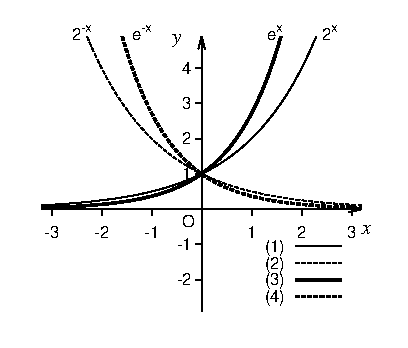
\includegraphics[width=8cm]{exp_2exp.eps}
%    \caption{問\ref{q:exp_graph0}の答え。}
%\end{figure}


\noindent{\textbf{答}}\ref{q:exp_evalue} 略 ($n=100$のとき$2.70\cdots$となる)。
\mv

%\noindent{\textbf{答}}\ref{q:def_NapierNum} 略 (がんばれ!)
\mv

\noindent{\textbf{答}}\ref{q:func_e_def} 略 ($n=10000$のとき$7.3875\cdots$
となる。それに対して, $e^2=7.3890\cdots$。)
\mv

% 金利2\%で100年間, お金を借りたときの
\noindent{\textbf{答}}\ref{q:func_exp_interest1} 略。どちらも最初の2桁は2.7になるはず。\mv

\noindent{\textbf{答}}\ref{q:func_exp_interest3} 
$(1+0.02)^{100}=(1+2/100)^{100}$の値を求めればよい。
\eref{eq:func_e_def}より, これは$e^2=7.38\cdots$に
近いはず。ちなみに, 厳密に計算すれば, $(1+0.02)^{100}=7.24\cdots$倍となる。
\mv

\noindent{\textbf{答}}\ref{q:func_exp_disaster} (1) $n$年に1回起きるのだから, 
今からの1年間がたまたまその1回にあたる確率は$1/n$。従って, あたらない
(豪雨が起きない)確率は$1-1/n$。(2) 「1年間で1回も起きない」が2回続くと考えて, 
$(1-1/n)^2$。(3)以降は略。\mv


\noindent{\textbf{答}}\ref{q:exp_graph1} 略。ヒント: $x=0$での$y$の
値をまず考えてみよう。その次に, $x$が$\infty$と$-\infty$に行く時の
それぞれについて, $y$の値がどうなっていくか考えてみよう。\\

\noindent{\textbf{答}}\ref{q:exp_diff0} 
\begin{edaenumerate}
\item $e^x$
\item $2e^{2x}$
\item $-2x\exp(-x^2)$
\item $(1-2x^2)\exp(-x^2)$
\end{edaenumerate}
\mv

\noindent{\textbf{答}}\ref{q:exp_log0} (略解)
\begin{enumerate}
\item 対数の定義より自明。
\item $a^1=a$より自明。
\item $a^0=1$より自明。
\item 
\begin{eqnarray*}a^{\log_a b+\log_a c}=a^{\log_a b}a^{\log_a c}=bc=a^{\log_a bc}\end{eqnarray*}
従って, $\log_a b+\log_a c=\log_a bc$\qed
\mv
\item $0=\log_a 1=\log_a \{b\times(1/b)\}=\log_a b+\log_a (1/b)$
従って, $\log_a (1/b)=-\log_a b$\qed
\mv
\item (4)(5)より明らか。
\item 左辺を指数として$a$の肩にのせると, (1)より, 
\begin{eqnarray*}a^{\log_a b^c}=b^c\end{eqnarray*}
一方, 右辺を指数として$a$の肩にのせると, 
\[a^{c\log_a b}=a^{(\log_a b)c}=\Bigl(a^{\log_a b}\Bigr)^c=b^c\]
これらは等しいから, 左辺=右辺。\qed
\mv
\item 左辺を指数として$a$の肩にのせると, 
\begin{eqnarray*}
a^{\log_a b \log_b c}=\Bigl(a^{\log_a b}\Bigr)^{\log_b c}=b^{\log_b c}=c
\end{eqnarray*}
一方, 右辺を指数として$a$の肩にのせると, 
\begin{eqnarray*}
a^{\log_a c}=c
\end{eqnarray*}
これらは等しいから, 左辺=右辺。\qed
\item \eref{eq:logloglog}で, $c$を$a$とおくと,
\begin{eqnarray*}(\log_a b) (\log_b a)=\log_a a=1\end{eqnarray*}
この両辺を$\log_b a$で割ると, 与式を得る。\qed
\item \eref{eq:logloglog}で, $a$を$c$, $b$を$a$, $c$を$b$におきかえると, 
\begin{eqnarray*}(\log_c a)(\log_a b)=\log_c b\end{eqnarray*}
この両辺を$\log_c a$で割ると, 与式を得る。\qed
\end{enumerate}
\mv

\noindent{\textbf{答}}\ref{q:exp_logvalue}
\begin{enumerate}
\item $\log_2 7=(\ln 7) / (\ln 2)\fallingdotseq2.807$
\item $\log_{0.3} 5=(\ln 5) / (\ln 0.3)\fallingdotseq -1.337$
\end{enumerate}
\mv

\noindent{\textbf{答}}\ref{q:exp_log_ln} 略。\eref{eq:logloglog}を使う。
\mv

\noindent{\textbf{答}}\ref{q:log10e_ln10} 略。(3)は\eref{eq:logloglog}を使う。
\mv

%\noindent{\textbf{答}}\ref{q:exp_logdif_num} 略。\mv

\noindent{\textbf{答}}\ref{q:exp_loggraph}  図\ref{fig:log_ln_ln1x_graph}参照。

\begin{figure}[h]
    \centering
      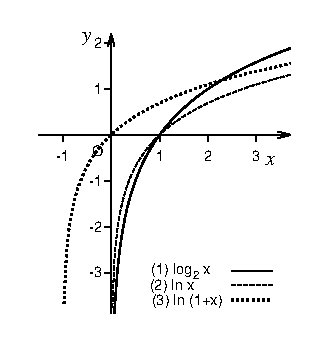
\includegraphics[width=7cm]{log2_ln.eps}
      \caption{問\ref{q:exp_loggraph}の答え。\label{fig:log_ln_ln1x_graph}}
\end{figure}

\noindent{\textbf{答}}\ref{q:exp_logdif0} 
\begin{enumerate}
\item $\frac{d}{dx}\ln(x+1)=\frac{1}{x+1}\times(x+1)'=\frac{1}{x+1}$
\item $\frac{d}{dx}\ln(2x)=\frac{1}{2x}\times(2x)'=\frac{1}{x}$
\item $0<x$のとき, $\frac{d}{dx}\ln|x|=\frac{d}{dx}\ln x = \frac{1}{x}$\\
$x<0$のとき, $\frac{d}{dx}\ln|x|=\frac{d}{dx}\ln(-x) = \frac{1}{-x}\times(-x)'=\frac{1}{-x}\times(-1)=\frac{1}{x}$\\
従って, $0<x$だろうが$x<0$だろうが, \\$\frac{d}{dx}\ln|x|=\frac{1}{x}$
\item $\frac{d}{dx}\ln(x-1)=\frac{1}{x-1}\times(x-1)'=\frac{1}{x-1}$
\item $\frac{d}{dx}\ln(1-x)=\frac{1}{1-x}\times(1-x)'=\frac{1}{1-x}\times(-1)=\frac{1}{x-1}$
\item $1<x$のとき, $\frac{d}{dx}\ln|1-x|=\frac{d}{dx}\ln (x-1) = \frac{1}{x-1}$ \\
$x<1$のとき, $\frac{d}{dx}\ln|1-x|=\frac{d}{dx}\ln(1-x) = \frac{1}{x-1}$ (前小問より)。
従って, $1<x$だろうが$x<1$だろうが, $\frac{d}{dx}\ln|1-x|=\frac{1}{x-1}$
\item $\frac{d}{dx}\ln \Bigl|\frac{x-1}{x+1}\Bigr|=\frac{d}{dx}(\ln |x-1|-\ln |x+1|)$\\
$=\frac{d}{dx}\ln |x-1|-\frac{d}{dx}\ln |x+1| = \frac{1}{x-1} - \frac{1}{x+1}=\frac{2}{x^2-1}$
\item (略解) $1/(x\ln 10)$
\end{enumerate}

\noindent{\textbf{答}}\ref{q:exp_diffxpowx} $f(x)=x^x$の両辺の対数をとると,\\
$\ln f(x)=x\ln x$。
この両辺を微分する。左辺の微分は$f'(x)/f(x)$。右辺の微分は
$\ln x+1$である。\\従って, $f'(x)/f(x)=\ln x+1$。\\従って, 
$f'(x)=(\ln x+1)f(x)=(1+\ln x)\,x^x$\qed
\vspace{0.3cm}

\noindent{\textbf{答}}\ref{q:exp_Gauss} $f(x)=\exp(-ax^2)$として($a$は実数の定数), 
\begin{enumerate}
\item $f(-x)=\exp\{-a(-x)^2\}=\exp(-ax^2)=f(x)$。従って偶関数。
\item $e=2.718\cdots$は0より大きいから, それを何乗しても0以下にはならない。
\item $f'(x)=-2ax\exp(-ax^2)$。これに$x=0$を代入すると0。
\item 
\begin{eqnarray}
\lim_{x\rightarrow\infty}\exp(-ax^2)=\lim_{x\rightarrow\infty}\frac{1}{e^{ax^2}}\label{eq:exp_Gauss_infty}
\end{eqnarray}
である。$0<a$だから, $x\rightarrow\infty$のとき, $ax^2\rightarrow\infty$である。
従って, $e^{ax^2}\rightarrow\infty$である。すなわち, \eref{eq:exp_Gauss_infty}
の右辺の分母は$\infty$に発散する。従って, \eref{eq:exp_Gauss_infty}は0に収束する。
\item $0\leq x$では, $e^{-ax^2}$は, 減少関数である。従って, $x=0$のとき最大値を
とる。$e^{-ax^2}$は偶関数なので, $x\leq 0$でも$x=0$のとき最大値をとる。従って, 
$e^{-ax^2}$は$x=0$のとき, 最大。
\end{enumerate}
\mv

\noindent{\textbf{答}}\ref{q:exp_Gauss_graph} 
\begin{enumerate}
\item 本文の図のとおり。
\item $\exp(-ax^2)=\exp\{-(\sqrt{a}\,x)^2\}$だから, $a$が大きくなると, グラフは$x$軸方向に
$1/\sqrt{a}$倍になる。つまり, 山型の幅が狭くなる。
\end{enumerate}
\mv

\noindent{\textbf{答}}\ref{q:exp_loglingraph0}  $(1, 0.5)$
\mv

\noindent{\textbf{答}}\ref{q:exp_loglingraph1} 略 
($a=0.69$, $A=0.25$程度になるはず(多少違っても構わない)。それを用いてS, T, Uの$y$の値を計算してみること)。
\mv

\noindent{\textbf{答}}\ref{q:exp_logloggraph0} 点Q: $(2, 7)$, 点R: $(0.2, 3)$
\mv

\noindent{\textbf{答}}\ref{q:exp_logloggraph1} 略 
($a=0.375$, $A=5.5$程度になるはず(多少違っても構わない)。それを用いてP, Q, Rの$y$の値を計算してみること。
$A$を求めるときの「切片」は, このグラフの左端ではなく, $x=1$のところの縦線に交わるときの値であることに注意)。
\mv

%解答: 
\noindent{\textbf{答}}\ref{q:exp_diffeq_sol00} (1) $f(x)=2x$として, 
\eref{eq:exp_diffeq_sol00}の左辺と右辺にそれぞれ代入すると, 
左辺=$(2x)'=2$, 右辺$=3(2x)=6x$となり, 左辺と右辺は恒等的には一致しない。
従って, この関数は\eref{eq:exp_diffeq_sol00}を満たさない(解ではない)。
(2)以下は略。(解であるのは(2), (4), (6)だけ)
\mv

%\noindent{\textbf{答}}\ref{q:exp_diffeq_sol20} 略。\mv

%% 放射性核種の崩壊
%\noindent{\textbf{答}}\ref{q:C14disint} 略。\mv

% \eref{eq:C14disint5}について, 
\noindent{\textbf{答}}\ref{q:funct_52} 
\begin{enumerate}
\item 図\ref{fig:Cchange}のとおり。
\begin{figure}
    \centering
    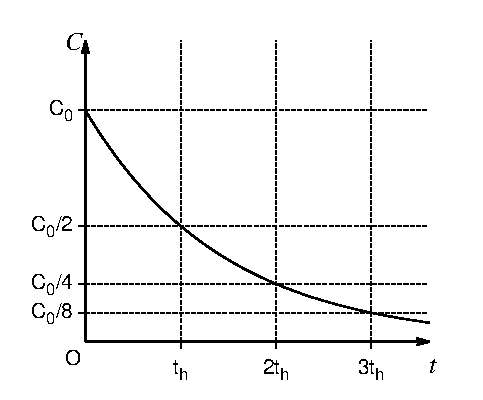
\includegraphics[width=8cm]{Cchange.eps}
    \caption{放射性炭素14の量の変化。\label{fig:Cchange}}
\end{figure}
\item 略。
\item 略解: $C=C_0 \exp[-(\ln 2) t/t_h]$   (導出過程も書くこと)
\item $\alpha=(\ln 2)/t_h$
\item $\alpha=(\ln 2)/(5730\text{年})\fallingdotseq1.21\times 10^{-4}$/年 ... 必ず単位を!
%\footnote{時定数は, 変化の約63パーセントが達成する時間であり, 半減期は変化の
%50パーセントが達成する時間である。従って, 常識的に考えて, 半減期より時定数の
%ほうが, 少し長い。}
\end{enumerate}
\mv

% 昔の火山噴火によってできた火山灰の地層の中から
\noindent{\textbf{答}}\ref{q:funct_54} $C=C_0/4$なので, $t=2t_h=11460$年くらい前(11500年でも可)。
\mv

%\begin{q}\label{q:funct_56} ある測定装置は, $C(0)$の1万分の1程度の不確かさで
%$C$を測ることができる。この装置で測れるのは, 何年くらい前までの試料か?\end{q}
%\hv
% ある測定装置は, $C_0$の1万分の1程度の不確かさで
%
%\noindent{\textbf{答}}\ref{q:funct_56} $C/C_0=(1/2)^{t/t_h}=1/10000$とすると, 
%$2^{t/t_h}=10000$だから, 
%$t/t_h=\log_2 10000=13.3$。従って, $t=13.3t_h\fallingdotseq$71000年程度。
%\hv

%\noindent{\textbf{答}}\ref{q:diffeq_1_chem_react} 略。\mv

%\noindent{\textbf{答}}\ref{q:logistic_func} 略。\mv

